\documentclass[a4paper,12pt]{article}
    \usepackage{listing}
    \usepackage{graphicx}
    \begin{document}
    \title{Second Readers-Writers Problem}
    \author{Santhisenan A}
    \date{\today}
    \maketitle
        
    \section{Readers-Writers Problem}
    In the readers-writers problem there are some processes ( termed readers ) who only read 
    the shared data, and never change it, and there are other processes ( termed writers ) 
    who may change the data in addition to or instead of reading it. There is no limit to how 
    many readers can access the data simultaneously, but when a writer accesses the data, 
    it needs exclusive access.
    
    
    The second readers-writers problem gives priority to the writers. In this problem, 
    when a writer wants access to the data it jumps to the head of the queue - All waiting readers
    are blocked, and the writer gets access to the data as soon as it becomes available. 
    In this solution the readers may be starved by a steady stream of writers.
    \subsection{Code}
        
    \begin{verbatim}
        import sys

        lock = 0
        no_of_readers = 0
        
        def reader():
            global no_of_readers
            print("Input: Reader")
            if lock:
                print("A wirter has acquired the lock, please wait till it releases the lock")
                return
            else:   
                no_of_readers += 1
                print("The reader can read.")
        
        def release_reader():
            global no_of_readers    
            if(no_of_readers == 0):
                print("No readers")
            else:
                no_of_readers -= 1
        
        def writer():
            global lock
            if lock:
                print("Another writer is reading.")
            else:
                print("Writer can write")
                lock = 1
        def release_writer():
            global lock
            if lock == 0:
                print("No writer is writing")
            else:
                lock = 0
        
        while True:
            read = input()
            if read == 'read':
                reader()
            elif read == 'write':
                writer()
            elif read == 'relread': # release reader
                release_reader()
            elif read == 'relwrite': # release writer
                release_writer()
            else: 
                sys.exit()        
    \end{verbatim}
    
\section{output}
\begin{figure}
    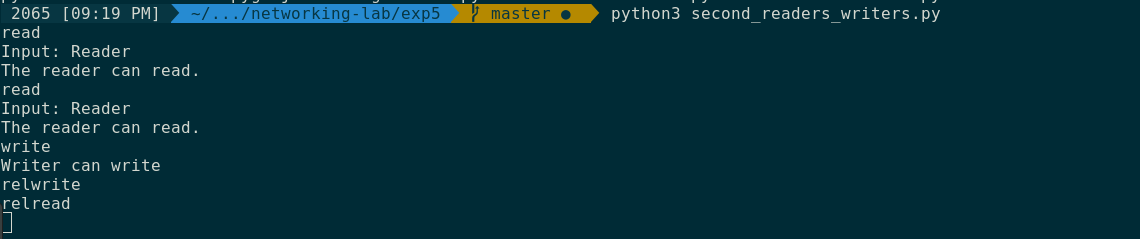
\includegraphics[width=\linewidth]{second-readers-writers.png}
    \caption{second-readers-writers}
    \end{figure}
\end{document}